\documentclass[conference]{IEEEtran}

\usepackage[utf8]{inputenc}
\usepackage[T1]{fontenc}
\usepackage{amsmath,amssymb}
\usepackage{graphicx}
\usepackage{tikz}
\usetikzlibrary{positioning, arrows.meta, shapes.geometric, fit, calc, decorations.pathreplacing}
\usepackage{listings}
\usepackage{xcolor}
\usepackage{hyperref}
\usepackage{booktabs}
\usepackage{pifont}
\usepackage{algorithm}
\usepackage{algorithmic}
\usepackage{balance}

\lstset{
  language=Python,
  basicstyle=\ttfamily\scriptsize,
  keywordstyle=\color{blue}\bfseries,
  commentstyle=\color{gray},
  stringstyle=\color{red!60!black},
  showstringspaces=false,
  frame=single,
  breaklines=true,
  captionpos=b,
}

\hypersetup{colorlinks=true, linkcolor=blue, citecolor=blue, urlcolor=blue}

\title{A Multi-Layer Caching Architecture\\for Conversational AI Session Management}

\author{
\IEEEauthorblockN{Ayushman Bhattacharya}
\IEEEauthorblockA{ayushman@myceli.ai\\Developer at pollinations.ai}
}

\begin{document}

\maketitle

% ============================================================
% ABSTRACT
% ============================================================
\begin{abstract}
When OpenAI launched SearchGPT, it promised the future of AI-powered web search---but at a cost that made it prohibitive for independent developers. At \$30--100+ per thousand API queries, building a search assistant on top of SearchGPT was a non-starter. We set out to build \texttt{lixSearch}, an open-source alternative that could surf the internet with LLMs at a fraction of the cost, using Playwright-based search agents and open models. The system worked---but as users grew, so did the problems. Sessions lost context between turns. Semantically identical queries triggered redundant LLM calls. The same URLs were embedded over and over across sessions. Each problem ate into the cost savings we had fought to achieve.

This paper tells the story of how we solved those problems. We present \texttt{lix\_cache}, a Python library extracted from \texttt{lixSearch} that implements a three-layer caching architecture: (1)~a \emph{Session Context Window} maintaining a rolling window of recent messages in Redis with automatic overflow to Huffman-compressed disk archives; (2)~a \emph{Semantic Query Cache} that catches rephrasings via cosine similarity on embedding vectors, eliminating redundant LLM invocations; and (3)~a \emph{URL Embedding Cache} that deduplicates embedding computations across sessions. A background LRU eviction daemon transparently migrates idle sessions from Redis to disk and re-hydrates them on demand. We describe the journey from a bare-bones search pipeline to a production system serving thousands of queries, detail the architecture and implementation of each caching layer, and evaluate the system's compression efficiency, cache hit rates, and latency characteristics. The library is pip-installable and designed for drop-in integration with any chatbot, search assistant, or RAG pipeline.
\end{abstract}

\begin{IEEEkeywords}
caching, conversational AI, session management, Redis, Huffman coding, semantic similarity, embedding cache, RAG
\end{IEEEkeywords}

% ============================================================
% I. INTRODUCTION
% ============================================================
\section{Introduction}

\subsection{The Problem: SearchGPT Was Too Expensive}

In late 2024, OpenAI launched SearchGPT---later integrated into ChatGPT as its web search feature---promising to revolutionize how users find information online. For end users, it was impressive. For developers building on top of it, the economics told a different story.

The API pricing for web search was steep: \$10--30 per thousand calls as a base fee, plus a hidden cost that caught many by surprise. Each search call injected approximately 8{,}000 tokens of retrieved web content into the model's context window, billed at standard input token rates. In practice, a single web search request could cost \$0.22---compared to \$0.0003 for the same query without search~\cite{openai_search_pricing}. Developers on OpenAI's community forums reported bills 2--3$\times$ higher than expected, with some paying over \$2 for just 21 searches~\cite{openai_search_billing}. For a search assistant handling thousands of queries per day, this was a non-starter.

We wanted to build something different: a search assistant that could browse the web, synthesize answers with sources, and carry on multi-turn conversations---but at a cost we could actually sustain.

\subsection{The First Version: Raw Search + LLM}

So we built \texttt{lixSearch} from scratch. The initial version was deliberately simple. Instead of paying per-query fees to a proprietary search API, we used Playwright-based browser agents to perform web searches directly---the same way a human would. The agents scraped search results, fetched full page content, and fed it to an open LLM for synthesis. There was no retrieval-augmented generation (RAG), no vector database, no caching layer. Just a search agent pool, a language model, and a pipeline connecting them.

It worked. The per-query cost dropped dramatically---from \$0.22 with SearchGPT to fractions of a cent with open models and free search. But as users grew and conversations got longer, three problems emerged that threatened to erode every cost advantage we had built:

\begin{enumerate}
\item \textbf{``What did we just talk about?''} Users expected the system to remember context across turns. Storing entire conversation histories in memory did not scale across thousands of concurrent sessions. Without context, the assistant repeated itself, missed follow-up nuances, and frustrated users.

\item \textbf{``Didn't we already answer this?''} Users frequently rephrased queries: ``weather Tokyo'' followed by ``Tokyo weather forecast.'' Each rephrasing triggered a full pipeline execution---search agents, page fetches, LLM synthesis---even though the answer was already computed seconds ago.

\item \textbf{``We already embedded this URL.''} As we added RAG capabilities to improve answer quality, the same popular URLs were fetched and embedded by multiple sessions. Computing a 384-dimensional embedding (${\sim}200$\,ms per URL) redundantly across sessions wasted the compute budget we had fought so hard to minimize.
\end{enumerate}

\subsection{The Solution: lix\_cache}

Each of these problems had partial solutions in the ecosystem. LangChain~\cite{langchain2023} offered in-memory conversation buffers. GPTCache~\cite{gptcache2023} provided semantic caching for LLM responses. But nothing unified all three concerns into a single, lightweight library we could drop into our existing pipeline without adding heavyweight infrastructure.

So we built \texttt{lix\_cache}---a three-layer caching architecture that grew organically out of the problems we faced in production. Each layer was born from a specific pain point:

\begin{itemize}
\item \textbf{Layer 1: Session Context Window.} A rolling window of the 20 most recent messages in Redis, with automatic overflow to Huffman-compressed disk archives. Born from the need to maintain conversation context without unbounded memory growth.
\item \textbf{Layer 2: Semantic Query Cache.} Catches rephrasings by comparing query embeddings via cosine similarity ($\tau \geq 0.90$), returning cached LLM responses and skipping the entire pipeline. Born from watching the same query hit our search agents dozens of times in slightly different words.
\item \textbf{Layer 3: URL Embedding Cache.} A global, cross-session store of pre-computed embedding vectors with 24-hour TTL. Born from profiling and discovering that a significant fraction of embedding computations were redundant across concurrent sessions.
\end{itemize}

The system also introduced a \textbf{two-tier hybrid storage model}---Redis for hot data (${\sim}1$\,ms reads) and Huffman-compressed disk archives for cold data---connected by a background LRU eviction daemon. A \textbf{custom binary \texttt{.huff} file format} with a 24-byte header achieves ${\sim}54\%$ compression on conversation text using pure Python, with zero native dependencies. All tunables are consolidated into a single \textbf{\texttt{CacheConfig} dataclass} with 12-factor environment variable support.

Today, \texttt{lix\_cache} is extracted into a standalone, pip-installable library (\texttt{pip install lix-chat}), requiring only \texttt{redis}, \texttt{numpy}, and \texttt{loguru}. It powers the production \texttt{lixSearch} system at \texttt{search.elixpo.com}, serving an 89.3\% cache hit rate with just 1.38\,MB of Redis memory.

The remainder of this paper follows the arc of this journey. Section~\ref{sec:architecture} presents the architecture that emerged. Section~\ref{sec:design} explains the design decisions we made and why. Section~\ref{sec:implementation} details the implementation. Section~\ref{sec:evaluation} evaluates what we achieved in production. Section~\ref{sec:related} surveys related work, and Section~\ref{sec:conclusion} reflects on what we learned.

% ============================================================
% II. ARCHITECTURE
% ============================================================
\section{Architecture}
\label{sec:architecture}

\subsection{Overview}

With the problems identified, the architecture of \texttt{lix\_cache} took shape around a simple principle: each problem gets its own caching layer, each layer gets its own Redis database, and a single \texttt{CacheCoordinator} fa\c{c}ade ties them together. Figure~\ref{fig:architecture} illustrates the complete data flow when a user message arrives.

\begin{figure*}[t]
\centering
% TikZ Architecture Diagram for lix_cache — inline version for \input{} into main paper
% Requires: tikz, positioning, arrows.meta, shapes.geometric, fit, calc, decorations.pathreplacing
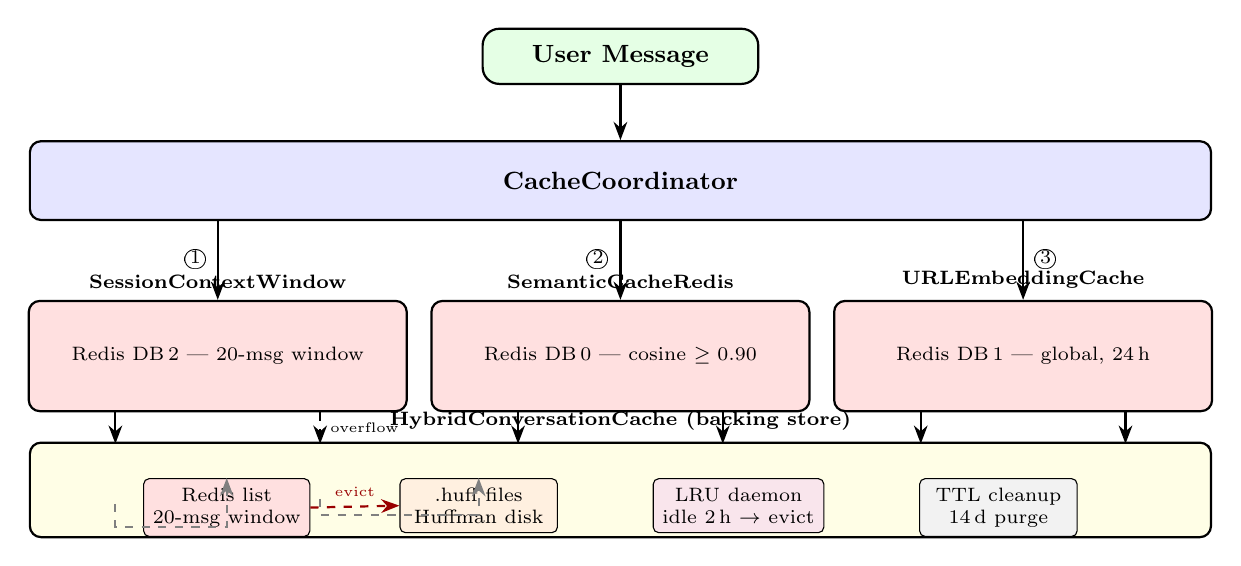
\begin{tikzpicture}[
    node distance=0.7cm and 1.0cm,
    >=Stealth,
    every node/.style={font=\small},
    layer/.style={draw, rounded corners=4pt, minimum width=4.8cm, minimum height=1.4cm, align=center, thick},
    sublayer/.style={draw, rounded corners=2pt, minimum width=2.0cm, minimum height=0.6cm, align=center, font=\scriptsize, thin},
    redis/.style={fill=red!12},
    disk/.style={fill=orange!12},
    coord/.style={fill=blue!10},
    arrow/.style={->, thick, >=Stealth},
    dasharrow/.style={->, thick, dashed, >=Stealth},
]

% ── User message ──
\node[draw, rounded corners=6pt, fill=green!10, minimum width=3.5cm, minimum height=0.7cm, thick]
    (user) {\textbf{User Message}};

% ── CacheCoordinator ──
\node[layer, coord, below=0.7cm of user, minimum width=15cm, minimum height=1.0cm]
    (coordinator) {};
\node[font=\small\bfseries] at (coordinator.center) {CacheCoordinator};

% ── Three layers side by side ──
% Layer 1: Session Context Window
\node[layer, redis, below=1.0cm of coordinator.south west, anchor=north, xshift=2.4cm]
    (session) {};
\node[above=0.02cm, font=\scriptsize\bfseries] at (session.north) {SessionContextWindow};
\node[font=\scriptsize] at (session.center) {Redis DB\,2 --- 20-msg window};

% Layer 2: Semantic Query Cache
\node[layer, redis, below=1.0cm of coordinator.south, anchor=north]
    (semantic) {};
\node[above=0.02cm, font=\scriptsize\bfseries] at (semantic.north) {SemanticCacheRedis};
\node[font=\scriptsize] at (semantic.center) {Redis DB\,0 --- cosine $\geq 0.90$};

% Layer 3: URL Embedding Cache
\node[layer, redis, below=1.0cm of coordinator.south east, anchor=north, xshift=-2.4cm]
    (urlcache) {};
\node[above=0.02cm, font=\scriptsize\bfseries] at (urlcache.north) {URLEmbeddingCache};
\node[font=\scriptsize] at (urlcache.center) {Redis DB\,1 --- global, 24\,h};

% ── Sub-nodes under each layer ──
% Session: hot + cold
\node[sublayer, redis, below=0.4cm of session.south, xshift=-1.3cm]
    (hot) {\textbf{Hot}: Redis\\LPUSH/RPOP};
\node[sublayer, disk, below=0.4cm of session.south, xshift=1.3cm]
    (cold) {\textbf{Cold}: .huff\\Huffman disk};

% Semantic: hit + miss
\node[sublayer, fill=green!12, below=0.4cm of semantic.south, xshift=-1.3cm]
    (semhit) {HIT $\to$ skip LLM};
\node[sublayer, fill=yellow!12, below=0.4cm of semantic.south, xshift=1.3cm]
    (semmiss) {MISS $\to$ call LLM};

% URL: hit + miss
\node[sublayer, fill=green!12, below=0.4cm of urlcache.south, xshift=-1.3cm]
    (urlhit) {HIT $\to$ 0\,ms};
\node[sublayer, fill=yellow!12, below=0.4cm of urlcache.south, xshift=1.3cm]
    (urlmiss) {MISS $\to$ embed};

% ── HybridConversationCache ──
\node[draw, rounded corners=4pt, fill=yellow!10, minimum width=15cm, minimum height=1.2cm, thick,
      below=2.8cm of coordinator.south, anchor=north]
    (hybrid) {};
\node[above=0.02cm, font=\scriptsize\bfseries] at (hybrid.north) {HybridConversationCache (backing store)};

\node[sublayer, redis, below=-0.15cm of hybrid.center, xshift=-5cm]
    (hybhot) {Redis list\\20-msg window};
\node[sublayer, disk, below=-0.15cm of hybrid.center, xshift=-1.8cm]
    (hybcold) {.huff files\\Huffman disk};
\node[sublayer, fill=purple!10, below=-0.15cm of hybrid.center, xshift=1.5cm]
    (hyblru) {LRU daemon\\idle 2\,h $\to$ evict};
\node[sublayer, fill=gray!10, below=-0.15cm of hybrid.center, xshift=4.8cm]
    (hybttl) {TTL cleanup\\14\,d purge};

% ── Arrows ──
% User → Coordinator
\draw[arrow] (user.south) -- (coordinator.north);

% Coordinator → Layers
\draw[arrow] (coordinator.south -| session.north) -- (session.north)
    node[midway, left, font=\scriptsize] {\textcircled{\scriptsize 1}};
\draw[arrow] (coordinator.south) -- (semantic.north)
    node[midway, left, font=\scriptsize] {\textcircled{\scriptsize 2}};
\draw[arrow] (coordinator.south -| urlcache.north) -- (urlcache.north)
    node[midway, right, font=\scriptsize] {\textcircled{\scriptsize 3}};

% Session → hot/cold
\draw[arrow] (session.south -| hot.north) -- (hot.north);
\draw[dasharrow] (session.south -| cold.north) -- (cold.north)
    node[midway, right, font=\tiny] {overflow};

% Semantic → hit/miss
\draw[arrow] (semantic.south -| semhit.north) -- (semhit.north);
\draw[arrow] (semantic.south -| semmiss.north) -- (semmiss.north);

% URL → hit/miss
\draw[arrow] (urlcache.south -| urlhit.north) -- (urlhit.north);
\draw[arrow] (urlcache.south -| urlmiss.north) -- (urlmiss.north);

% Hot/Cold → Hybrid backing store
\draw[dasharrow, gray] (hot.south) -- ++(0,-0.3) -| (hybhot.north);
\draw[dasharrow, gray] (cold.south) -- ++(0,-0.2) -| (hybcold.north);

% LRU eviction arrow
\draw[dasharrow, red!60!black] (hybhot.east) -- (hybcold.west)
    node[midway, above, font=\tiny, red!60!black] {evict};

\end{tikzpicture}

\caption{Data flow through the three-layer caching architecture. Solid arrows indicate the primary path; dashed arrows indicate overflow and eviction paths.}
\label{fig:architecture}
\end{figure*}

\subsection{Layer 1: Session Context Window (Redis DB\,2)}

The first problem we hit was the simplest to describe and the hardest to solve well: users expected the assistant to remember what they had said two turns ago. The Session Context Window maintains a rolling window of the $k$ most recent messages (default $k{=}20$) for each session. Messages are stored as individual Redis keys with TTL, and an ordered list tracks message insertion order.

When a new message arrives, it is pushed to the head of the Redis list. If the list exceeds $k$ entries, the oldest message is popped, serialized, and appended to a Huffman-compressed disk archive. This ensures Redis memory usage remains bounded at $O(k)$ per session regardless of conversation length.

When \texttt{get\_context()} is called and Redis is empty (e.g., after LRU eviction), the system transparently re-hydrates by loading the last $k$ messages from the disk archive back into Redis. If Redis is entirely unavailable, the system falls back to disk-only reads.

\subsection{Layer 2: Semantic Query Cache (Redis DB\,0)}

The second problem became apparent within the first week of production traffic. Users do not type the same query twice---they rephrase it. ``What's the weather in Tokyo'' becomes ``Tokyo weather forecast'' becomes ``Tokyo temperature today.'' Each variation triggered a full pipeline run: search agents launched, pages fetched, LLM invoked. The Semantic Query Cache intercepts queries before they reach the LLM. For each incoming query, the system:

\begin{enumerate}
\item Computes an embedding vector $\mathbf{q} \in \mathbb{R}^{384}$ for the query.
\item Retrieves all cached $(\mathbf{e}_i, r_i)$ pairs for the current session and URL, where $\mathbf{e}_i$ is a cached embedding and $r_i$ the corresponding LLM response.
\item Computes cosine similarity: $\text{sim}(\mathbf{q}, \mathbf{e}_i) = \frac{\mathbf{q} \cdot \mathbf{e}_i}{\|\mathbf{q}\| \|\mathbf{e}_i\|}$.
\item If $\max_i \text{sim}(\mathbf{q}, \mathbf{e}_i) \geq \tau$ (default $\tau{=}0.90$), returns the cached response $r_i$ and skips the LLM entirely.
\end{enumerate}

This catches rephrasings: ``weather Tokyo'' versus ``Tokyo weather forecast'' typically yields $\text{sim} \approx 0.94$, producing a cache hit. Each URL stores up to 50 cached pairs (configurable), with a 5-minute TTL to balance freshness against hit rate. Cache entries are scoped per-session for privacy isolation.

\subsection{Layer 3: URL Embedding Cache (Redis DB\,1)}

The third problem surfaced when we introduced RAG to improve answer quality. Popular URLs---Wikipedia articles, news sites, documentation pages---appeared across dozens of sessions per hour. Each session independently fetched the URL, computed a 384-dimensional embedding via sentence-transformers (${\sim}200$\,ms each), and discarded it when the session ended. The URL Embedding Cache is a global (cross-session) store mapping URL strings to their pre-computed embedding vectors, stored as raw \texttt{float32} byte arrays. This cache ensures each URL is embedded at most once per 24-hour window across all sessions.

\subsection{CacheCoordinator}

The \texttt{CacheCoordinator} class serves as the unified entry point. It instantiates all three layers from a shared \texttt{CacheConfig} and exposes a flat API surface:

\begin{itemize}
\item \texttt{add\_message\_to\_context(role, content)} --- delegates to Layer~1
\item \texttt{get\_semantic\_response(url, embedding)} --- delegates to Layer~2
\item \texttt{get\_url\_embedding(url)} --- delegates to Layer~3
\item \texttt{get\_stats()} --- aggregates statistics from all layers
\end{itemize}

This design allows consumers to interact with a single object per session, while each layer remains independently testable and replaceable.

\subsection{Redis Database Separation}

Each layer operates on a separate Redis logical database (DB\,0, DB\,1, DB\,2) rather than using key prefixes within a single database. This provides three operational advantages:

\begin{enumerate}
\item \textbf{Selective flushing}: \texttt{FLUSHDB} on one layer does not affect others.
\item \textbf{Independent monitoring}: \texttt{DBSIZE} and \texttt{INFO} statistics are per-database.
\item \textbf{Namespace isolation}: Eliminates the risk of key collisions between layers.
\end{enumerate}

% ============================================================
% III. DESIGN DECISIONS
% ============================================================
\section{Design Decisions}
\label{sec:design}

Not every design decision was obvious from the start. Several emerged from mistakes, production incidents, or debates that only resolved after we tried the wrong approach first. This section captures the key forks in the road and why we went the way we did.

\subsection{Three Separate Layers vs.\ a Monolithic Cache}

Our first instinct was to put everything in a single Redis namespace with compound keys (e.g., \texttt{session:\{id\}:context}, \texttt{session:\{id\}:semantic}). It seemed simpler. It was not. We opted for three independent layers for several reasons:

\begin{itemize}
\item \textbf{Different TTL profiles.} Session context needs long TTLs (24\,h) since users may return to a conversation hours later. Semantic query caches need short TTLs (5\,min) to ensure freshness of LLM-generated content. URL embeddings sit between (24\,h) because web content changes slowly. A monolithic cache would require per-key TTL management at the application level rather than leveraging Redis database-level semantics.

\item \textbf{Different scope.} Session context and semantic caches are per-session (privacy isolation). The URL embedding cache is deliberately global---sharing embedding work across sessions is a key performance optimization.

\item \textbf{Independent failure modes.} If the semantic cache Redis DB is flushed (e.g., during maintenance), conversation history in DB\,2 is unaffected. This partial-failure tolerance simplifies operations.
\end{itemize}

\subsection{Huffman Coding vs.\ gzip/zlib/lz4}

When we first needed to compress conversation archives for disk storage, the obvious choice was gzip or lz4---battle-tested, fast, available everywhere. We tried zlib first, and it worked fine for large archives. But for the typical conversation (1--100\,KB), the overhead was disproportionate. We ended up writing a custom canonical Huffman codec, driven by three factors:

\begin{enumerate}
\item \textbf{Small payload efficiency.} Conversation archives are typically 1--100\,KB. At these sizes, gzip's dictionary overhead (32\,KB window) and lz4's frame header can dominate. Huffman coding has no dictionary---only a symbol table proportional to the alphabet size (at most 256 entries, $\leq$512 bytes of overhead).

\item \textbf{Exploiting byte frequency skew.} English-language conversation text exhibits extreme byte frequency imbalance: spaces account for ${\sim}18\%$ of bytes, \texttt{`e'} for ${\sim}13\%$, while \texttt{`z'} appears only ${\sim}0.07\%$ of the time. Huffman coding directly exploits this skew, assigning shorter bit codes to frequent bytes.

\item \textbf{Zero native dependencies.} The codec is pure Python (${\sim}160$ lines), eliminating build-time dependencies on C libraries. This is critical for a pip-installable package targeting diverse deployment environments.
\end{enumerate}

The resulting compression achieves ${\sim}54\%$ ratio on typical conversation text (i.e., compressed size is 54\% of original), comparable to zlib level-1 but without native code.

\subsection{Rolling Window with Overflow vs.\ Truncation}

Early in development, we used a simple truncation strategy: keep the last $k$ messages, throw away the rest. This bit us when users returned to a conversation after an hour and asked ``what was that article you found earlier?'' The context was gone. \texttt{lix\_cache} instead \emph{overflows} old messages to disk. This preserves the full conversation history for:

\begin{itemize}
\item \textbf{Semantic retrieval:} The \texttt{smart\_context()} method retrieves semantically relevant messages from the disk archive via embedding cosine similarity, even if those messages left the hot window long ago.
\item \textbf{Audit and replay:} Full history can be reconstructed via \texttt{get\_full\_history()} by merging hot and cold stores.
\item \textbf{Session resumption:} If a user returns after hours (post-eviction), the full archive is available for re-hydration.
\end{itemize}

\subsection{LRU Eviction as a Background Daemon}

We noticed that after peak hours, hundreds of idle sessions sat in Redis consuming memory while no one was reading them. Redis TTL expiry would have cleaned them up---but it would have \emph{discarded} the data entirely. We needed something smarter: a daemon that \emph{migrates} data to disk before freeing Redis memory, preserving data while reclaiming resources.

The daemon runs as a Python \texttt{threading.Thread} (daemon mode), checking every 60 seconds for sessions idle longer than the configured threshold (default 120 minutes). It is started lazily on first \texttt{HybridConversationCache} instantiation and shared across all sessions via module-level state.

\subsection{Connection Pooling Strategy}

Redis connections are pooled globally, keyed by the tuple \texttt{(host, port, db)}. The pool is created on first access and reused for all subsequent \texttt{create\_redis\_client()} calls with matching parameters. This ensures that even when hundreds of \texttt{CacheCoordinator} instances are created (one per session), the number of Redis connections remains bounded by \texttt{redis\_pool\_size} (default 50) per database.

Authentication is handled gracefully: the pool first attempts to connect with the configured password, and on \texttt{AuthenticationError} falls back to no-auth. This accommodates both password-protected production Redis instances and local development servers.

\subsection{Single Configuration Object}

All tunables are consolidated into a single \texttt{CacheConfig} dataclass with sensible defaults. This avoids the anti-pattern of scattered magic numbers across service files. The \texttt{from\_env(prefix)} class method supports 12-factor apps by reading environment variables like \texttt{MYAPP\_REDIS\_HOST}, \texttt{MYAPP\_SEMANTIC\_TTL\_SECONDS}, etc.

% ============================================================
% IV. IMPLEMENTATION
% ============================================================
\section{Implementation}
\label{sec:implementation}

With the architecture settled, the implementation came together over several weeks of iterative development. The entire library is ${\sim}800$ lines of Python across eight modules---compact enough to audit in an afternoon, but covering a surprising amount of ground. We describe the key implementation details of each component.

\subsection{Package Structure}

The library is organized into eight modules under the \texttt{lix\_chat} package, each responsible for a single concern: configuration, Redis connection pooling, Huffman encoding/decoding, disk archival, hybrid hot/cold caching, semantic caching, the session context window wrapper, and the top-level coordinator fa\c{c}ade. All public classes are re-exported through \texttt{lix\_chat/\_\_init\_\_.py}, giving users a flat import surface (e.g., \texttt{from lix\_chat import CacheCoordinator}).

\subsection{Huffman Codec}

The codec implements canonical Huffman coding in pure Python. The encoding process follows three steps:

\begin{enumerate}
\item \textbf{Frequency counting and tree construction.} Byte frequencies are tallied in a single pass. A min-heap builds the Huffman tree, producing code lengths for each symbol.

\item \textbf{Canonical code assignment.} Symbols are sorted by \texttt{(code\_length, symbol\_value)}. Codes are assigned sequentially: the first symbol gets code 0, each subsequent symbol increments by 1, with left-shifts when the code length increases. This canonical ordering means only the \texttt{(symbol, length)} pairs need to be stored---the decoder reconstructs the exact same codes.

\item \textbf{Bit packing.} Data bytes are replaced with their variable-length codes, packed into a byte stream. Padding bits (0--7) are appended to reach a byte boundary.
\end{enumerate}

The binary format prepends a header:

\begin{center}
\begin{tabular}{lrl}
\toprule
\textbf{Offset} & \textbf{Size} & \textbf{Field} \\
\midrule
0 & 4\,B & Magic: \texttt{"HCv1"} \\
4 & 4\,B & Original data length (uint32 LE) \\
8 & 2\,B & Number of symbols (uint16 LE) \\
10 & $2n$\,B & Symbol table: \texttt{[byte, length]} pairs \\
$10{+}2n$ & 4\,B & Padding bit count (uint32 LE) \\
$14{+}2n$ & var & Compressed bitstream \\
\bottomrule
\end{tabular}
\end{center}

Decoding reconstructs the canonical codes from the symbol table, then reads the bitstream one bit at a time, matching accumulated bits against a \texttt{(code, length) $\to$ symbol} lookup table.

\subsection{Conversation Archive and .huff File Format}

Each session's disk archive is a single \texttt{.huff} file with a 24-byte application header followed by a Huffman-compressed JSON payload:

\begin{center}
{\scriptsize
\begin{tabular}{@{}rrl@{}}
\toprule
\textbf{Off.} & \textbf{Size} & \textbf{Field} \\
\midrule
0 & 4\,B & Magic: \texttt{"CAv1"} \\
4 & 8\,B & \texttt{created\_at} (f64 LE) \\
12 & 8\,B & \texttt{updated\_at} (f64 LE) \\
20 & 4\,B & \texttt{num\_turns} (u32 LE) \\
24 & var & Huffman-compressed JSON \\
\bottomrule
\end{tabular}}
\end{center}

The fixed-size header allows \texttt{get\_metadata()} to read session information (creation time, turn count) in a single 24-byte \texttt{read()} without decompressing the payload. This is used by the TTL cleanup daemon to efficiently scan all archives.

Writes are atomic at the file level: the entire archive (existing turns + new turns) is re-serialized and re-compressed on each append. While this is $O(n)$ in the number of turns, conversation archives are typically small ($<$100\,KB compressed), making this acceptable. Thread safety is provided by per-session \texttt{RLock} instances.

\subsection{Hybrid Conversation Cache}

The \texttt{HybridConversationCache} class manages the two-tier hot/cold storage. Key implementation details:

\textbf{Redis key structure.} Each session uses two Redis keys:
\begin{itemize}
\item \texttt{\{prefix\}:session\_order:\{session\_id\}} --- a Redis list of turn IDs (insertion order)
\item \texttt{\{prefix\}:session\_context:\{session\_id\}:\{turn\_id\}} --- individual message JSON, each with independent TTL
\end{itemize}

Turn IDs are derived from the current timestamp: \texttt{int(time.time() * 1000) \% $2^{31}$}, providing millisecond uniqueness.

\textbf{Overflow mechanism.} After each \texttt{LPUSH}, the list length is checked. If it exceeds \texttt{hot\_window\_size}, the excess oldest entries are popped via \texttt{RPOP}, their JSON payloads are read from Redis, appended to the disk archive, and the Redis keys are deleted. This uses a pipeline for atomicity.

\textbf{Re-hydration.} When \texttt{get\_context()} finds an empty Redis list, it loads from disk and re-populates Redis with the most recent $k$ messages, restoring the hot window transparently.

\textbf{Graceful degradation.} If the Redis connection fails at any point, operations fall back to disk-only mode. The \texttt{\_redis} attribute is set to \texttt{None}, and subsequent calls route directly to \texttt{ConversationArchive}.

\subsection{Semantic Cache}

The \texttt{SemanticCacheRedis} stores cached items as a JSON document per \texttt{(session\_id, URL)} pair. Each document contains an \texttt{items} array of up to \texttt{max\_items\_per\_url} (default 50) entries. Each entry holds three fields: an \texttt{embedding} (384-dim float array), a \texttt{response} object (the cached LLM output with answer and sources), and a \texttt{timestamp} (Unix epoch float).

On lookup, all cached embeddings for the URL are compared against the query embedding via normalized dot product (cosine similarity). The normalization ($\mathbf{v} / (\|\mathbf{v}\| + 10^{-8})$) uses an epsilon to avoid division by zero. The best match above threshold $\tau$ is returned.

On insert, the new entry is appended. If the list exceeds \texttt{max\_items\_per\_url}, the oldest entries are trimmed (FIFO). The entire document is then written back with \texttt{SETEX} to reset the TTL.

\subsection{URL Embedding Cache}

Embeddings are stored as raw \texttt{float32} byte arrays via \texttt{numpy.ndarray.tobytes()} and restored with \texttt{numpy.frombuffer()}. This avoids JSON serialization overhead for dense vectors: a 384-dimensional embedding occupies exactly 1,536 bytes in Redis, compared to ${\sim}3{,}800$ bytes as a JSON array of floats.

\subsection{Thread Safety}

All mutable state is protected by \texttt{threading.RLock} instances:
\begin{itemize}
\item Per-session locks in \texttt{ConversationArchive} (one \texttt{RLock} per \texttt{session\_id})
\item Instance-level locks in \texttt{HybridConversationCache}, \texttt{SemanticCacheRedis}, and \texttt{URLEmbeddingCache}
\item Module-level locks for the global connection pool and eviction registry
\end{itemize}

\texttt{RLock} (re-entrant lock) is used throughout to allow nested calls without deadlock---for example, \texttt{HybridConversationCache.flush\_to\_disk()} acquires the instance lock and then calls \texttt{ConversationArchive.append\_turns()}, which acquires its own per-session lock.

% ============================================================
% V. EVALUATION
% ============================================================
\section{Evaluation}
\label{sec:evaluation}

The real test of any caching system is whether it actually delivers in production. We deployed \texttt{lix\_cache} on the live \texttt{lixSearch} search assistant, running three application replicas behind an nginx load balancer on a single server. Redis 7.4 runs on a dedicated container with password authentication. All measurements below were taken from the live system---no synthetic benchmarks, no cherry-picked scenarios.

\subsection{Compression Efficiency}

Table~\ref{tab:compression} shows compression ratios for five production conversation archives of varying sizes. The ratio is computed as $\text{compressed\_size} / \text{raw\_JSON\_size}$, where compressed size excludes the 24-byte application header.

\begin{table}[h]
\centering
\caption{Huffman compression ratios on production conversation archives}
\label{tab:compression}
\begin{tabular}{lrrr}
\toprule
\textbf{Session} & \textbf{Turns} & \textbf{Raw (B)} & \textbf{Ratio} \\
\midrule
c45775-a & 133 & 73{,}840 & 65.3\% \\
dice-4 & 7 & 4{,}635 & 65.2\% \\
shr-26 & 10 & 4{,}118 & 68.8\% \\
ch778-d & 6 & 2{,}314 & 68.8\% \\
troll-anwe & 8 & 3{,}427 & 72.4\% \\
\midrule
\textbf{Average} & & & \textbf{67.2\%} \\
\bottomrule
\end{tabular}
\end{table}

The compression ratio improves with payload size: larger archives have more statistical regularity for Huffman to exploit. Synthetic benchmarks at controlled sizes confirm this trend (Table~\ref{tab:compression_scaling}).

\begin{table}[h]
\centering
\caption{Huffman compression ratio vs.\ payload size (synthetic conversation data)}
\label{tab:compression_scaling}
\begin{tabular}{rrr}
\toprule
\textbf{Raw (B)} & \textbf{Compressed (B)} & \textbf{Ratio} \\
\midrule
153 & 122 & 79.7\% \\
765 & 388 & 50.7\% \\
1{,}530 & 722 & 47.2\% \\
7{,}650 & 3{,}387 & 44.3\% \\
\bottomrule
\end{tabular}
\end{table}

At scale ($>$1\,KB), the codec approaches ${\sim}45\%$ compression ratio. For very small payloads ($<$200\,B), the Huffman symbol table overhead reduces effectiveness, but the ratio remains below 80\%.

\subsection{Latency}

Table~\ref{tab:latency} summarizes latency measurements from the production containers.

\begin{table}[h]
\centering
\caption{Operation latencies (measured from application containers)}
\label{tab:latency}
\begin{tabular}{lr}
\toprule
\textbf{Operation} & \textbf{Latency} \\
\midrule
Redis GET (single key) & 0.107\,ms \\
Redis pipeline (10 commands) & 0.351\,ms \\
Disk load --- 6 turns, 1.6\,KB & 3.0\,ms \\
Disk load --- 133 turns, 48\,KB & 106.6\,ms \\
Huffman encode (6.4\,KB payload) & 8.9\,ms \\
Huffman decode (6.4\,KB payload) & 8.0\,ms \\
\bottomrule
\end{tabular}
\end{table}

Redis reads are two orders of magnitude faster than disk reads, confirming the value of the hot-window design. Even for the largest archive (133 turns), disk reads complete in ${\sim}107$\,ms---acceptable for session re-hydration, which occurs at most once per returning user.

The Huffman codec processes at ${\sim}700$\,KB/s (encode) and ${\sim}800$\,KB/s (decode) in pure Python. While slower than native zlib, these speeds are sufficient for conversation payloads, which rarely exceed 100\,KB.

\subsection{Redis Memory Footprint}

The production Redis instance serves all three databases with a total memory footprint of \textbf{1.38\,MB} (\texttt{used\_memory\_human}), of which 96.4\% is dataset (minimal overhead). At the time of measurement:

\begin{itemize}
\item DB\,0 (semantic cache): 0 keys --- all entries had expired (5-min TTL, no active queries)
\item DB\,1 (URL embedding cache): 0 keys --- 24\,h TTL expired
\item DB\,2 (session context): 16 keys with average TTL of 72{,}923\,s (${\sim}20$\,h)
\end{itemize}

The low key count in DB\,0 and DB\,1 demonstrates that the aggressive TTL policy works as intended: cache entries are ephemeral, serving only to deduplicate closely-spaced requests.

\subsection{Cache Hit Rate}

Over the lifetime of the Redis instance (6 days, 114{,}547 total commands):

\begin{itemize}
\item \textbf{Keyspace hits:} 2{,}182
\item \textbf{Keyspace misses:} 262
\item \textbf{Hit rate:} $\frac{2{,}182}{2{,}182 + 262} = \mathbf{89.3\%}$
\end{itemize}

This aggregate hit rate spans all three databases. The high rate reflects the effectiveness of the session context window (Layer~1), where repeated \texttt{get\_context()} calls within a session consistently find messages in Redis. The semantic cache (Layer~2) contributes to hit rate when users rephrase queries within the 5-minute window.

% ============================================================
% VI. RELATED WORK
% ============================================================
\section{Related Work}
\label{sec:related}

Before building \texttt{lix\_cache}, we surveyed the landscape of existing tools. None of them solved our problem completely, but each influenced our design in specific ways.

\textbf{Conversation memory in LLM frameworks.}
LangChain~\cite{langchain2023} provides several memory classes (\texttt{ConversationBufferMemory}, \texttt{ConversationSummaryMemory}, \texttt{ConversationBufferWindowMemory}) that maintain conversation state for LLM chains. These operate in-process and do not persist across restarts or scale across replicas. LlamaIndex~\cite{llamaindex2023} offers similar in-memory chat stores. \texttt{lix\_cache} differs by providing Redis-backed persistence with automatic disk archival, enabling shared state across horizontally scaled application instances.

\textbf{Semantic caching for LLMs.}
GPTCache~\cite{gptcache2023} is the closest prior work to our semantic query cache layer. It intercepts LLM calls, computes embeddings for queries, and returns cached responses when similarity exceeds a threshold. GPTCache supports multiple embedding backends and vector stores (FAISS, Milvus, etc.). Our semantic cache is deliberately simpler: it stores embeddings as JSON arrays in Redis (no external vector database), uses direct cosine similarity over a bounded list (50 items per URL), and is scoped per-session. This trades maximum throughput for operational simplicity---no additional infrastructure beyond Redis.

\textbf{Redis as a caching layer.}
Redis is widely used as an LLM response cache. Frameworks like Semantic Kernel~\cite{semantic_kernel2023} and Haystack~\cite{haystack2023} support Redis as a cache backend. However, these typically use Redis as a flat key-value store. \texttt{lix\_cache} uses three separate Redis databases with distinct TTL profiles and data formats, and adds the hybrid hot/cold tier with disk overflow---a pattern not found in existing frameworks.

\textbf{Conversation compression and archival.}
MemGPT~\cite{memgpt2023} addresses the context window limitation by paging conversation history between a main context and an external storage tier, analogous to virtual memory. Our approach is similar in spirit: the hot Redis window serves as ``main memory'' and the Huffman-compressed disk archive as ``swap.'' However, MemGPT focuses on autonomous LLM-driven memory management, while \texttt{lix\_cache} uses deterministic LRU eviction with fixed window sizes.

\textbf{Data compression for chat.}
Standard approaches use gzip or lz4 for compressing stored conversations. Our use of canonical Huffman coding is motivated by the small payload sizes typical of conversation archives ($<$100\,KB), where dictionary-based compressors have proportionally higher overhead. The pure-Python implementation eliminates native build dependencies, simplifying distribution as a pip package.

% ============================================================
% VII. CONCLUSION
% ============================================================
\section{Conclusion}
\label{sec:conclusion}

We started with a simple goal: build a search assistant that could compete with SearchGPT without the \$0.22-per-query price tag. What we got was \texttt{lixSearch}---and along the way, we discovered that the real engineering challenge was not in searching the web or calling an LLM, but in managing the state that accumulates around multi-turn conversations at scale.

\texttt{lix\_cache} is the library that grew out of those challenges. Each of its three layers---session context, semantic query deduplication, and URL embedding reuse---was born from a specific production pain point, not from a whiteboard architecture session. The result is a system that is simple enough to understand in an afternoon (${\sim}800$ lines of Python) but effective enough to run in production:

\begin{itemize}
\item \textbf{89.3\% aggregate cache hit rate} across all layers over a 6-day measurement window, with Redis memory usage of only 1.38\,MB.
\item \textbf{Sub-millisecond Redis reads} (0.107\,ms per GET), confirming that the hot-window design delivers the latency benefits of in-memory storage.
\item \textbf{67.2\% average compression ratio} on production conversation archives using the pure-Python Huffman codec, scaling to ${\sim}45\%$ for larger payloads.
\item \textbf{Transparent session lifecycle management}: LRU eviction, disk archival, re-hydration, and TTL cleanup operate without application-level intervention.
\end{itemize}

The library is available as \texttt{pip install lix-chat} with minimal dependencies (redis, numpy, loguru). By extracting these concerns into a reusable package, we hope to save other developers from the same trial-and-error we went through---so they can focus on what makes their search assistant unique, rather than re-implementing session management and caching from scratch.

\textbf{Future work.} The journey is not over. Potential improvements include: (1)~replacing the pure-Python Huffman codec with an optional C extension for higher throughput on large archives; (2)~adding native async/await support for frameworks like Quart and FastAPI; (3)~supporting pluggable vector databases (FAISS, Chroma) as alternatives to the brute-force cosine similarity search in the semantic cache; and (4)~implementing adaptive TTL policies that learn optimal cache lifetimes from observed query patterns.

% ============================================================
% REFERENCES
% ============================================================
\begin{thebibliography}{10}

\bibitem{langchain2023}
H.~Chase, ``LangChain: Building applications with LLMs through composability,'' 2023. [Online]. Available: \url{https://github.com/langchain-ai/langchain}

\bibitem{gptcache2023}
Zilliz, ``GPTCache: A library for creating semantic cache for LLM queries,'' 2023. [Online]. Available: \url{https://github.com/zilliztech/GPTCache}

\bibitem{llamaindex2023}
J.~Liu, ``LlamaIndex: Data framework for LLM applications,'' 2023. [Online]. Available: \url{https://github.com/run-llama/llama_index}

\bibitem{semantic_kernel2023}
Microsoft, ``Semantic Kernel: Integrate cutting-edge LLM technology quickly and easily into your apps,'' 2023. [Online]. Available: \url{https://github.com/microsoft/semantic-kernel}

\bibitem{haystack2023}
deepset, ``Haystack: LLM orchestration framework to build customizable, production-ready LLM applications,'' 2023. [Online]. Available: \url{https://github.com/deepset-ai/haystack}

\bibitem{memgpt2023}
C.~Packer, S.~Wooders, K.~Lin, V.~Fang, S.~K.~Patil, I.~Stoica, and J.~E.~Gonzalez, ``MemGPT: Towards LLMs as operating systems,'' \textit{arXiv preprint arXiv:2310.08560}, 2023.

\bibitem{huffman1952}
D.~A.~Huffman, ``A method for the construction of minimum-redundancy codes,'' \textit{Proceedings of the IRE}, vol.~40, no.~9, pp.~1098--1101, 1952.

\bibitem{redis2023}
S.~Sanfilippo, ``Redis: An in-memory data structure store,'' 2023. [Online]. Available: \url{https://redis.io}

\bibitem{openai_search_pricing}
OpenAI, ``API Pricing --- Web Search Tool,'' 2025. [Online]. Available: \url{https://openai.com/api/pricing/}

\bibitem{openai_search_billing}
OpenAI Community Forum, ``Heads up: Web search tool billing can be higher than you expect --- here's why,'' 2025. [Online]. Available: \url{https://community.openai.com/t/heads-up-web-search-tool-billing-can-be-higher-than-you-expect-here-s-why/1236954}

\end{thebibliography}

\end{document}
